\documentclass{beamer}
\usetheme{Darmstadt}
\usepackage{beamerthemesplit}
\usepackage{latexsym}
\usepackage{ae,aecompl}
\usepackage{graphicx}
\usepackage{amsfonts}
\usepackage{tikz}
\usepackage{graphics}
\usepackage{url}
\usepackage{booktabs}

\graphicspath{{../images/}}

\hypersetup{
  pdftitle={MSWL Project Evaluation: OpenNebula Project Analysis},
  pdfauthor={Sergio Arroutbi Braojos},
  pdfcreator={},
  pdfproducer=PDFLaTeX,
  pdfsubject={nn},
}

\title{MSWL Project Evaluation: OpenNebula Project Analysis}
\author{Sergio Arroutbi Braojos}
\begin{document}
% Background Image
\setbeamertemplate{background}{%
    \tikz\node[opacity=0.1] at (current page.center) {
    \vbox to \paperheight{\vfil\hbox to \paperwidth{\hfil
\includegraphics[width=6cm]{opennebula.png}\hfil}\vfil}
 };
}
\frame{\titlepage
\begin{flushright}
{\tiny
(cc) 2014 Sergio Arroutbi Braojos.
    This work is under a license Creative Commons CC-BY 3.0.\\
To view a copy of full license, see \url{http://creativecommons.org/licenses/by/3.0/}
}
\begin{figure}[h]
    \begin{flushright}	
        
\includegraphics[width=0.6in]{by.png}
        \label{fig:by}
    \end{flushright}
\end{figure}
\end{flushright}
}

%\section[Index]{}
%\begin{frame}[allowframebreaks]
%\tableofcontents
%\end{frame}

\section{About}

% Presentation
\begin{frame}[allowframebreaks]
\frametitle{About OpenNebula}

\begin{itemize}
	\item FLOSS Cloud Computing Framework:\linebreak
	- Flexible Enterprise Cloud Made Simple\linebreak
	- Mission: Simple but feature-rich and flexible solution to build and manage enterprise clouds and virtualized data centers\linebreak
 - Main Objective: Lead innovation in enterprise-class cloud data center management\linebreak
 - Core Values: 
   \begin{enumerate}\itemsep0pt
   \item{Openness}
   \item{Excellence}
   \item{Cooperation}
   \item{Innovation}
   \end{enumerate}
	\item Project Start: 2008\\
 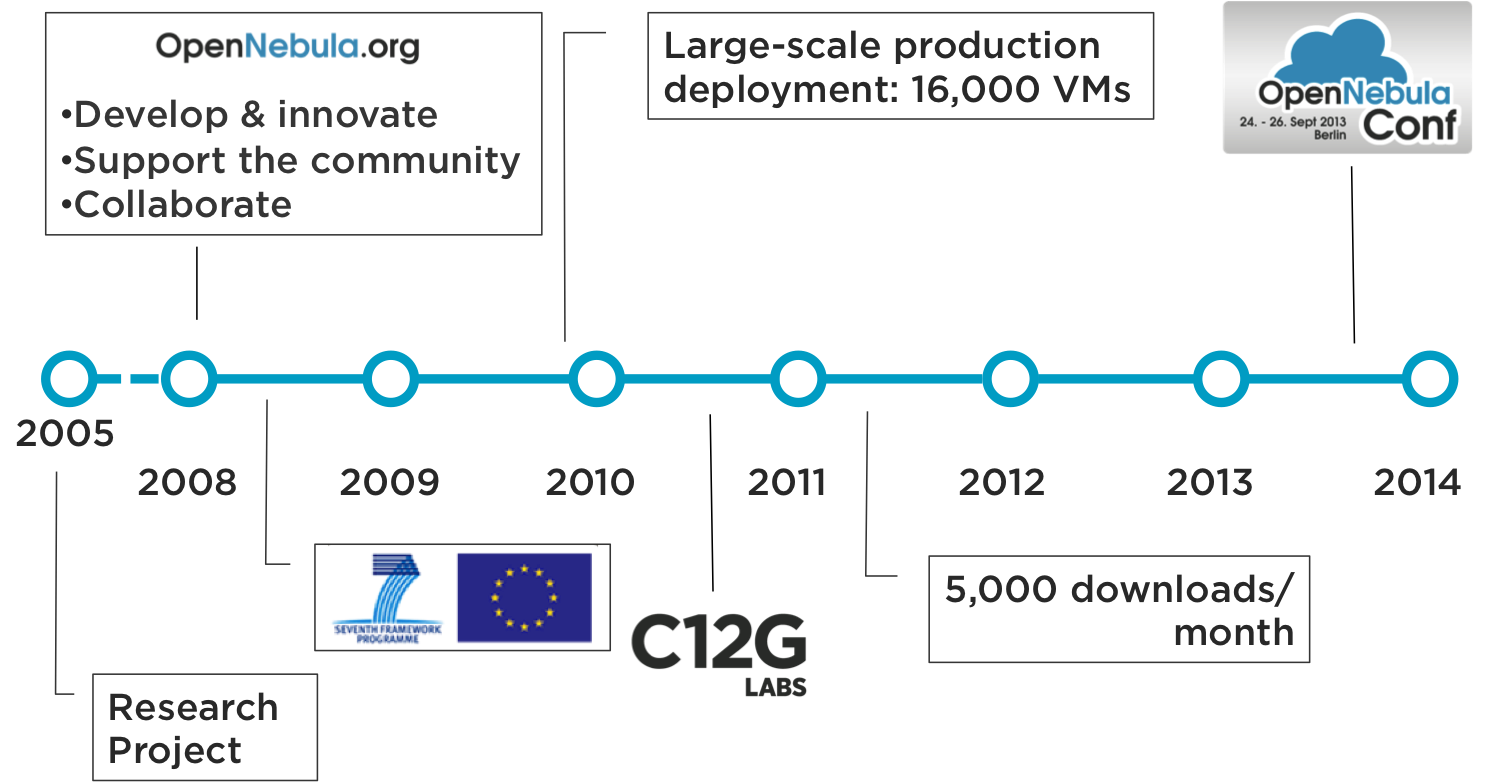
\includegraphics[width=4in]{opennebula-history.png}
\end{itemize}

\end{frame}

\section{Art State}

% Presentation
\begin{frame}[allowframebreaks]
\frametitle{Cloud Computing State of the Art }

\begin{itemize}
	\item OpenNebula \\
	- CG12 Labs, Focused on Functionality, Weak Community
	\item CloudStack \\
	- Open CloudStack, by Apache (Community, Openness)
	\item Eucalyptus \\ 
	- OpenSource AWS Compatible Private Clouds
	\item OpenStack \\
	- More than 200 hundred companies involved
\end{itemize}

\end{frame}

\section{Objectives}

% Origin
\begin{frame}[allowframebreaks]
\frametitle{Objectives}

"Find which Cloud Computing Open Source Project has more
Quality according to an evaluator necessities" \linebreak
Methodology followed to identify the most
appropriate Cloud Computing Open Source Project:
\begin{itemize}
	\item Candidates Identification (State of Art)
	\item Define Quality Model (OpenBRR based)
	\item Invent evaluator role, defining necessities => Weights
	\item Analyse a project (OpenNebula)
        \item Compare with competitor projects (OpenStack,
        Eucalyptus, CloudStack)
\end{itemize}

\end{frame}

\section{Quality Model}

\begin{frame}[allowframebreaks]
\frametitle{Quality Model}
\begin{itemize}\itemsep0pt
\item{OpenBRR based.} Spreadsheet available.
\item{Model: 2 Levels.} Categories + metrics.
\item{Categories:}
\begin{enumerate}
	\item Functionality (5 metrics)
	\item Efficiency, Benchmarks (2 metrics)
	\item Professional Support (1 metric)
	\item Documentation (2 metrics)
        \item Community (3 metrics)
\end{enumerate}
\item{Weights: 2 Levels as well}:
\begin{enumerate}
	\item Category weights (Importance of category)
	\item Inside category weights (Importance of each
          metric inside a category)
\end{enumerate}
\end{itemize}

\end{frame}

\section{Role}

\begin{frame}[allowframebreaks]
\frametitle{Role}
\begin{itemize}\itemsep0pt
\item{Open Source background}
\item{Community First}
\item{Functionality ``comes'' with community}
\item{Category weights:}
\begin{enumerate}
	\item Functionality (10\%)
	\item Efficiency, Benchmarks (15\%)
	\item Professional Support (20\%)
	\item Documentation (25\%)
        \item Community (30\%)
\end{enumerate}
\item{Inside category metric weights}:
\begin{enumerate}
	\item All aspects important inside category
	\item No special considerations
        \item 1 Metric (100\%), 2 Metrics (50/50\%), 3
          Metrics (33/33/33\%), 4 Metris (25/25/25/25\%), ...
\end{enumerate}
\end{itemize}

\end{frame}

\section{Analysis}

\begin{frame}[allowframebreaks]
\frametitle{Analysis}
Tools used:
\begin{itemize}\itemsep0pt
\item{OpenNebula Web Portal}. Functionality. Professional Support.
\item{Google}. Efficiency.
\item{cvsanaly2}. Documentation and Community.
\end{itemize}
Data Sources:
\begin{itemize}\itemsep0pt
\item{Documentation associated to Key Features on OpenNebula project}.
\item{Documentation associated to Commercial Support}.
\item{OpenStack/OpenNebula benchmark comparison}.
\item{OpenNebula ``one'' Git repository}.
\end{itemize}

\end{frame}

\section{Results}

\begin{frame}[allowframebreaks]
\frametitle{Results}

\begin{table}[H]
  \begin{center}
    \begin{tabular}{ | p{3cm} | p{2.5cm} | p{1.5cm} | p{2cm} | }
    \toprule
    \textbf{Category} & \textbf{Unweighted Rating} & \textbf{Weight} & \textbf{Weighted Score}\\
    \hline
    Functionality & 4.2 & 10\% & 0.42\\
    \hline
    Efficiency & 2 & 15\% & 0.3\\
    \hline
    Support & 3 & 20\% & 0.6\\
    \hline
    Documentation & 4 & 25\% & 1\\
    \hline
    Community & 2.33 & 30\% & 0.7\\
    \midrule
    \textbf{Final Score} & \multicolumn {3}{c|}{\textbf{3.02}}\\
    \bottomrule
    \end{tabular}
    \caption{OpenNebula Score}
    \label{tab:final_score}
  \end{center}
\end{table}

\end{frame}

\section{Comparison}

\begin{frame}[allowframebreaks]
\frametitle{Comparison}

\begin{table}[H]
  \begin{center}
    \begin{tabular}{ | p{2cm} | p{1cm} | p{1cm} | p{1cm} | p{1cm} | p{1cm} | p{1cm} | }
    \toprule
    Project & \textbf{Final Score} & Func. & Effic. & Supp. & Doc. & Comm.\\
    \hline
    CloudStack & \textbf{3.57} & 0.38 & 0.45 & 0.6 & 1.25 & 0.891\\
    \hline
    Eucalyptus & \textbf{3.43} & 0.46 & 0.45 & 0.6 & 1.13 & 0.79\\
    \hline
    OpenStack & \textbf{3.31} & 0.34 & 0.45 & 1 & 1.13 & 0.4\\
    \hline
    OpenNebula & \textbf{3.02} & 0.42 & 0.3 & 0.6 & 1 & 0.7\\
    \midrule
    \textbf{Winner Project} & \multicolumn {6}{c|}{\textbf{CloudStack}}\\
    \bottomrule
    \end{tabular}
    \caption{Comparison Table}
    \label{tab:comparison_table}
  \end{center}
\end{table}

\end{frame}

\begin{frame}
\frametitle{References}

% Just for format reference

\begin{itemize}
\tiny{
\item Angela Byron, Drupal 7 maintainer, ``Drupal Community Demystified''
 \url{http://www.youtube.com/watch?v=PSjkRJ2mM54}

\item Stephanie Torres, ``Drupal Association Board Meeting''
 \url{https://association.drupal.org/node/18208}

\item Drupal Maintainers
 \url{https://api.drupal.org/api/drupal/MAINTAINERS.txt}

\item DrupalCon
 \url{https://drupal.org/drupalcon}

} %tiny
\end{itemize}

\end{frame}


\end{document}
